%%%%%%%%%%%%%%%%%%%%%%%%%%%%%%%%%%%%%%%
%
% Cosas  a revisar:
% the data / data (i.e., "we need data to be complete")
%
%%%%%%%%%%%%%%%%%%%%%%%%%%%%%%%%%%%%%%%%
%\textcolor{red}{TODO: Recordar poner que P(x) es lo mismo que P(X=x)}
%
%\textcolor{red}{TODO: En aprendizaje hablo de descomposicion pero no lo nombro en ningun otro momento. Deberia introducir ese termino antes de aprendizaje, a partir de la definicion del modelo.}
%
%Al terminar, leermelo entero y repasar la notacion. Que sea consistente de inicio a fin.
%
%Habria que ver que el tono es el mismo en todo el capitulo, hay secciones como la de aprendizaje que tienen un enfoque mas de explicacion y otros como el de inferencia que es mas estilo SoTA

%%%%%%%%%%%%%%%%%%%%%%%%%%%%%%%%%%%%%%%%
\chapter{Bayesian networks} \label{ch:2_bayesian_networks}
\section{Introduction}
Most real-world problems imply dealing with uncertainty. This is a consequence of several factors such as partial information, stochastic environments, and measurement errors. Probability theory provides a well-established foundation for managing uncertainty, therefore it is natural to use it for reasoning under these conditions. However, if we naïvely apply probability to complex problems, we will soon be deterred by the resulting computational complexity \citep{sucar2015}.

PGMs provide a computationally efficient framework for managing uncertainty that combines probability theory with graph theory. The main idea is to consider only those conditional probabilistic independence relations that are held in the problem data and encode them in a graph. By using a PGM, we can compactly and clearly represent the JPD of the data, graphically representing relevant relationships between the problem variables. We distinguish two components in a PGM: the graphical structure and the probabilistic content. In the graphical structure, nodes correspond to random variables and arcs correspond to probabilistic dependences between them. The probabilistic content quantifies these dependences using CPDs. The JPD is factorized according to the graphical structure as a product of those CPDs, which reduces the total number of model parameters and facilitates the computation of probabilistic queries.

Depending on the type of graphical structure, we can distinguish three main families of PGMs: (i) Markov networks \citep{kidermann1980}, which assume an undirected graph to represent relations between the problem variables, (ii) BNs \citep{pearl1988}, which assume a directed acyclic graph, and (iii) chain graphs \citep{lauritzen1989}, which admit both directed and undirected arcs, but without any directed cycles. In this dissertation, we mainly work with BNs, as they are the most widely used PGM for reasoning with uncertainty. They are commonly used in fields as diverse as medical diagnosis \citep{pourret2008}, maintenance planning \citep{jones2010}, risk assessment \citep{fenton2012}, neuroscience \citep{bielza2014} and many more \citep{koller2009}. 

\subsection*{Chapter outline}
In Section \ref{sec:2_bayesian_network_model}, we start with a brief overview of how a graph can encode conditional independence relations and then formally introduce the BN model with its parametrizations. In Section \ref{sec:2_inference}, we present the mechanism of probabilistic inference. Finally, in Section \ref{sec:2_learning}, we overview the problem of learning BNs, where we put especial attention in explaining the differences between the complete and incomplete data case.

\section{The Bayesian network model} \label{sec:2_bayesian_network_model}
A BN is a compact representation of a JPD over a set of random variables. We can distinguish two components in a BN: (i) a directed acyclic graphical structure that encodes conditional independence relations between the different variables, and (ii) a set of parameters that, together with the graphical structure, define a unique distribution. We start with a brief overview of how a graph encodes the conditional independence relations and then formally define the BN model with its parametrizations.

\subsection{Encoding independences}
At the core of BNs is the concept of conditional independence. Let $P$ be a probability distribution with $\mathbf{X}_{A}$, $\mathbf{X}_{B}$ and $\mathbf{X}_{C}$ as three disjoint sets of variables. We say that $\mathbf{X}_{A}$ and $\mathbf{X}_{B}$ are conditionally independent given $\mathbf{X}_{C}$ if
\begin{equation*}
P(\mathbf{X}_{A}, \mathbf{X}_{B} | \mathbf{X}_{C}) = P(\mathbf{X}_{A} | \mathbf{X}_{C}) P (\mathbf{X}_{B} | \mathbf{X}_{C}) \ 
\end{equation*}
and we denote this statement by $(\mathbf{X}_{A} \perp \mathbf{X}_{B} | \mathbf{X}_{C})$. As an example, the BN structure depicted in Figure \ref{fig:2_bn_example} implies several conditional independence statements over its set of variables $\{X_{1}, X_{2}, X_{3}, X_{4}, X_{5}\}$: $(X_{1} \perp X_{2})$, $(X_{3} \perp \{X_{2}, X_{4}\} | X_{1})$, $(X_{4} \perp \{X_{3}, X_{5}\}| \{X_{1}, X_{2}\})$ and $(X_{5} \perp \{X_{1}, X_{2}, X_{4}\} | X_{3})$. We see a pattern emerging from the independence statements of this example: the parents of a variable ``shield" it from the probabilistic influence of other variables that are not its descendants. We can formalize this intuition. 

Let $\mathcal{G}$ be a DAG whose nodes represent a set of random variables $\mathbf{X}$. Let $\mathbf{Pa}_{i}^{\mathcal{G}}$ denote the parents of $X_{i}$ in $\mathcal{G}$, and $\text{NonDescendants}_{X_{i}}$ denote the variables in the graph that are nondescendants of $X_{i}$. Then $\mathcal{G}$ encodes the following set of conditional independence statements, called the local Markov independences, and denoted by $\mathcal{I}_{l}(\mathcal{G})$:
\begin{equation*}
\forall X_{i} : \ (X_{i} \perp \text{NonDescendants}_{X_{i}} | \mathbf{Pa}_{i}^{\mathcal{G}}) \ .
\end{equation*}

\begin{figure}[t!]
	\begin{center}
		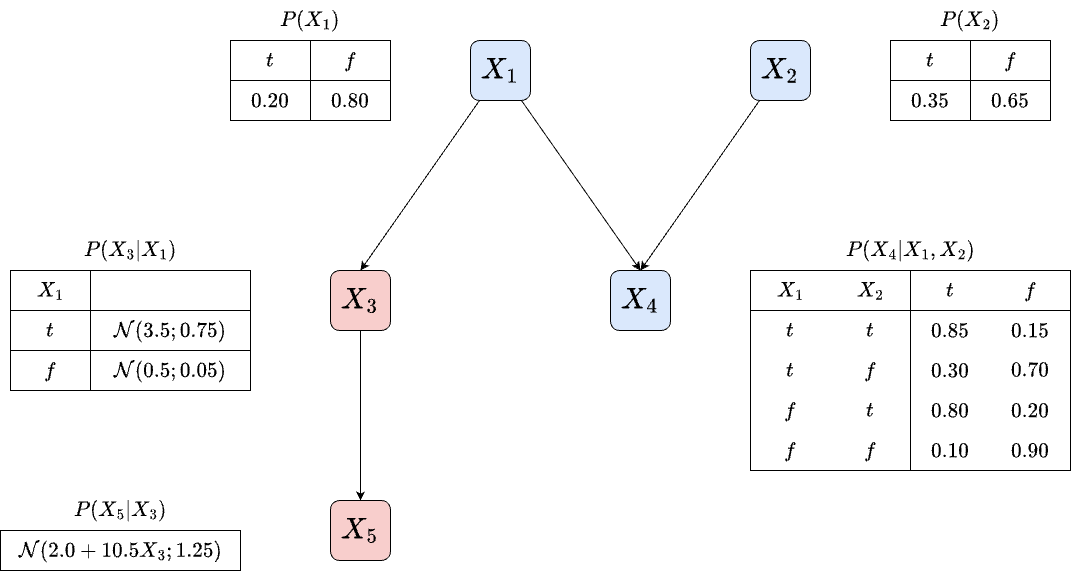
\includegraphics[width = \textwidth]{2_bayesian_networks/figures/bn_example.pdf}
		\caption{Example of a conditional linear Gaussian BN. Blue nodes represent categorical variables and red nodes represent continuous variables.}
		\label{fig:2_bn_example}
	\end{center}
\end{figure}

The ability to infer conditional independences from a graph allows us to characterize the notion of Markov blanket (MB). The MB of any variable $X_{i} \in \mathbf{X}$ in $\mathcal{G}$ is the set of variables composed of the parents of $X_{i}$, its children and the parents of its children.

In general there are multiple conditional independence statements that can be derived from $\mathcal{I}_{l}(\mathcal{G})$. The notion of d-separation can be used to determine whether a specific statement $(\mathbf{X}_{A} \perp \mathbf{X}_{B} | \mathbf{X}_{C})$ holds. Let $\mathbf{X}_{A}$, $\mathbf{X}_{B}$ and $\mathbf{X}_{C}$ be three disjoint sets of nodes in a DAG $\mathcal{G}$. Let $\mathbf{T}$ be the set of possible trials from any node $X_{a} \in \mathbf{X}_{A}$ to any node $X_{b} \in \mathbf{X}_{B}$, where a trial in the graph is a succession of arcs, independent of their directions. Then $\mathbf{X}_{C}$ blocks a trial $T_{I} \in \mathbf{T}$ if one of the following holds:
\begin{enumerate}
	\item $T_{I}$ contains a chain $T_{i-1} \rightarrow T_{i} \rightarrow T_{i+1}$ such that $T_{i} \in \mathbf{X}_{C}$.
	\item $T_{I}$ contains a fork $T_{i-1} \leftarrow T_{i} \rightarrow T_{i+1}$ such that $T_{i} \in \mathbf{X}_{C}$.
	\item $T_{I}$ contains a collider $T_{i-1} \rightarrow T_{i} \leftarrow T_{i+1}$ such that $T_{i}$ and any of its descendants do not belong to $\mathbf{X}_{C}$.
\end{enumerate}

If all the trials in $\mathbf{T}$ are blocked by $\mathbf{X}_{C}$, then $\mathbf{X}_{C}$ d-separates $\mathbf{X}_{A}$ and $\mathbf{X}_{B}$. It is important to note that d-separation does not rule out additional conditional independences that may hold in the distribution and are not encoded by the DAG. For example, if $\mathbf{X}_{A}$ and $\mathbf{X}_{B}$ are d-separated given $\mathbf{X}_{C}$, then $(\mathbf{X}_{A} \perp \mathbf{X}_{B} | \mathbf{X}_{C})$ holds in the distribution $P$. However, a lack of d-separation does not necessarily indicate that $(\mathbf{X}_{A} \perp \mathbf{X}_{B} | \mathbf{X}_{C})$ does not hold in $P$. Finally, d-separation can be efficiently computed in time that is linear in the number of nodes in the graph \citep{geiger1990}.

%If all the trials in $\mathbf{T}$ are blocked by $\mathbf{X}_{C}$, then $\mathbf{X}_{C}$ d-separates $\mathbf{X}_{A}$ and $\mathbf{X}_{B}$. D-separation can be efficiently computed in time that is linear in the number of nodes in the graph \citep{geiger1990}. It is important to note that d-separation only tells us about conditional independences that must follow from the graph that encodes $\mathcal{I}_{l} (\mathcal{G})$. That is, if $\mathbf{X}_{A}$ and $\mathbf{X}_{B}$ are d-separated given $\mathbf{X}_{C}$, then $(\mathbf{X}_{A} \perp \mathbf{X}_{B} | \mathbf{X}_{C})$ holds in the distribution $P$. However, a lack of d-separation does not necessarily indicate that $(\mathbf{X}_{A} \perp \mathbf{X}_{B} | \mathbf{X}_{C})$ does not hold in $P$. D-separation does not rule out additional conditional independences that may hold in $P$ and are not encoded in the graph structure.

Since we are interested in DAGs that encode a JPD, we now define the relation between the topological properties of a DAG and the conditional independences  of its underlying probability distribution. We say that a DAG $\mathcal{G}$ is an independence map (I-map) of the distribution $P$ if all the conditional independences that can be derived from $\mathcal{I}_{l}(\mathcal{G})$ are satisfied by $P$. We can now formally define the BN model.

\subsection{Model definition}
A BN $\mathcal{B} = (\mathcal{G}, \bm{\theta})$ is a representation of a JPD over a set of random variables $\mathbf{X}$. It consists of two components: (i) a DAG $\mathcal{G}$ that encodes the conditional independences $\mathcal{I}_{l}(\mathcal{G})$, and (ii) a set of parameters $\bm{\theta}$ that describes the CPD $P(X_{i} | \mathbf{Pa}^{\mathcal{G}}_{i})$ of each variable $X_{i} \in \mathbf{X}$ given its parents in the graph. In addition, we require that $\mathcal{G}$ is an I-map of the JPD $P$ represented by the BN. This property is key for allowing the BN to compactly factorize the JPD as a product of CPDs. It is formally expressed by the following theorem:
\begin{thm}
	{\normalfont\citep{pearl1988}} Let $\mathcal{G}$ be a BN graph over the set of variables $\mathbf{X}$. We say that $\mathcal{G}$ is an I-map of $P$ if and only if $P$ can be expressed as
	\begin{equation}
	\label{eq:bn_jpd}
	P(\mathbf{X}) = \prod_{i} P(X_{i} | \mathbf{Pa}_{i}^{\mathcal{G}}) \ .
	\end{equation}
\end{thm}
Using this theorem, a BN is able to define a unique probability distribution that can be written as in Equation (\ref{eq:bn_jpd}). This is called the chain rule for Bayesian networks. As an example, consider the distribution $P(X_{1},X_{2},X_{3},X_{4},X_{5})$ of Figure \ref{fig:2_bn_example}. By taking into account the conditional independences represented by the graph, we can write:
\begin{equation*}
P(X_{1},X_{2},X_{3},X_{4},X_{5}) = P(X_{1})P(X_{2})P(X_{3}|X_{1})P(X_{4}|X_{1},X_{2})P(X_{5}|X_{3}) \ .
\end{equation*}

\subsection{Parametrization}
Depending on the nature of variables that are present in a BN, we usually distinguish between categorical, continuous, and hybrid (i.e., mixed) BNs. The latter is composed of both categorical and continuous variables. Each of these is presented in the following sections.

\subsubsection{Categorical Bayesian networks}

Categorical BNs are strictly composed of categorical variables (i.e., qualitative variables with a finite number of values). Examples include variables such as sex, eye color, blood type, and many others. However, discrete variables with a finite number of values can also be used (e.g., number of children in a family, number of tests in an experiment, etc.). The terms ``categorical" and ``discrete" are usually used indiscriminately in the BN literature. For simplicity, we are going to refer to both types of variables as categorical variables. The natural choice for modelling categorical variables is the categorical distribution. The categorical distribution is a generalization of the Bernoulli distribution that allows more than two possible values. This distribution provides several advantages to categorical BNs. First, all of the CPDs are categorical distributions, which simplifies computations. Second, each CPD can be represented in tabular form, where every assignment of a variable and its parents has a designated probability. Third, they are easily interpretable due to a direct representation of the BN parameters as probabilities. All these benefits make categorical BNs the most common parametrization in the literature \citep{darwiche2009}. 

%For simplicity, finite discrete variables are usually considered categorical variables.
%
%For simplicity, we are going to refer to this type of discrete variables as categorical variables. 

%Categorical BNs are strictly composed of categorical variables (i.e., each variable has a finite number of values). Examples include variables such as sex, eye color, blood type, and many others. The natural choice for modelling categorical variables is the categorical distribution. The categorical distribution is a generalization of the Bernoulli distribution that allows more than two possible values. This distribution provides several advantages to categorical BNs. First, all of the CPDs are categorical distributions, which simplifies computations. Second, each CPD can be represented in tabular form, where every assignment of a variable and its parents has a designated probability. Third, they are easily interpretable due to a direct representation of the BN parameters as probabilities. All these benefits make categorical BNs the most common parametrization in the literature \citep{darwiche2009}. 

As an example, consider the CPD $P(X_{4}|X_{1}, X_{2})$ of Figure \ref{fig:2_bn_example}. In this example, $X_{4}$ takes two possible values $\{t,f\}$, and their respective probabilities depend on the assignment of parent variables $X_{1}$ and $X_{2}$. One problem, however, arises from using this representation: the number of parameters in a categorical CPD increases exponentially with respect to the number of parents, which limits the complexity of the model.



%As an example, consider the CPD $P(X_{4}|X_{1}, X_{2})$ of Figure \ref{fig:2_bn_example}. In this example, $X_{4}$ has a categorical distribution with four values, each one corresponding to an assignment of $X_{1}$ and $X_{2}$. One problem, however, arises from using this representation: the number of parameters in a categorical CPD increases exponentially with respect to the number of parents, which limits the complexity of the model.

\subsubsection{Continuous Bayesian networks}
Continuous BNs are strictly composed of continuous variables (i.e., quantitative variables with an uncountable number of values). Examples include variables such as age, weight, blood pressure and many others. In this section, we describe how continuous variables can be integrated into the BN framework. We first describe the discretization approach, which simply transforms continuous variables into categorical variables. Then, we present the linear Gaussian BN, which is composed of linear Gaussian CPDs and it is the most commonly used approach. Finally, we comment several semiparametric and nonparametric approaches that are not based on the Gaussian distribution.

\subsubsection*{Discretization}
Given the desirable properties of categorical BNs, it is natural to bin continuous variables into a finite set of intervals. Two types of discretization techniques can be distinguished \citep{fu2005}:
\begin{itemize}
	\item Prediscretization methods, which discretize the data prior to the definition or learning of the BN. Due to the pertinence of these methods to most machine learning algorithms, a great deal of research has focused on this area \citep{liu2002}.
	\item Integrated methods, which employ a greedy iterative search that alternates between BN structure learning and discretization. They are more computationally expensive than prediscretization methods, but they have also shown better results at modelling the data \citep{friedman1996_disc, monti1999}.
\end{itemize}

Discretization is still an active research topic and different strategies can be applied to different types of data \citep{nojavan2017, beuzen2018}. The main drawback of discretizing continuous variables is that it unavoidably results in loss of information. All variation within the created intervals is discarded. As a consequence, certain dependences between variables may become unnoticeable \citep{friedman2000_disc}.

\subsubsection*{Linear Gaussian Bayesian networks}
The most commonly used parametric form for continuous density functions is the Gaussian distribution. The Gaussian distribution is a member of the exponential family \citep{wainwright2008} that makes very strong assumptions, such as the exponential decay of the distribution away from its mean, and the linearity of interactions between its variables. While these assumptions are often invalid, the Gaussian distribution has proven to be a surprisingly good approximation for many real-world distributions \citep{kotz2004}.

In a linear Gaussian BN \citep{shachter1989_gauss}, all of its variables are continuous and all of its CPDs are linear Gaussians. Let $X$ be a continuous variable with continuous parents $\mathbf{C} = \{C_{1},\dots, C_{k}\}$. We say that $X$ has a linear Gaussian CPD if there are parameters $\beta_{0},\dots,\beta_{k}$ and $\sigma^{2}$ such that
\begin{equation*}
P(X|\mathbf{C}) = \mathcal{N}(\beta_{0} + \sum_{i=1}^{k}\beta_{k}C_{i}; \sigma^{2}) \ .
\end{equation*}

From this formulation we can see that $X$ follows a Gaussian distribution with a mean that is linear in the values of its parent variables $\mathbf{C}$ and with a variance $\sigma^{2}$. An important result of this formulation is that linear Gaussian BNs are an alternative representation for the class of multivariate Gaussian distributions and vice versa. As an example, consider the conditional distribution $P(X_{5}|X_{3})$ of Figure \ref{fig:2_bn_example}. In this example, $X_{5}$ has a  continuous parent, $X_{3}$, and follows a linear Gaussian distribution with parameters $\beta_{0} = 2.0$, $\beta_{1} = 10.5$ and $\sigma^{2} = 1.25$. Linear Gaussian BNs are widely used in the continuous domain due to their support of efficient inference \citep{koller2009} and learning \citep{geiger1994_bge}.
\subsubsection*{Other approaches}
Some researchers have investigated the use of richer (semiparametric or nonparametric) models for representing nonlinear dependencies in BNs with continuous variables. These include kernel estimators \citep{hofmann1995}, neural networks \citep{monti1997,choi2018}, and Gaussian processes \citep{friedman2000_gp}. While these approaches may result in a better representation of the underlying probability distribution, they have several disadvantages: (i) they are harder to interpret due to their use of models that are opaque to humans, and (ii) they do not usually allow efficient inference or learning.
\subsubsection{Hybrid Bayesian networks}
Hybrid BNs are composed of both categorical and continuous variables. So far we have discussed the relations between variables of the same type, categorical or continuous. We have shown that in the case of categorical variables, the categorical distribution is the natural CPD. In addition, for continuous variables, we have shown the advantages of the linear Gaussian CPD. We can extrapolate this knowledge to hybrid BNs when both the parents and the children are categorical or continuous. However, there are two new types of relations that we need to address: (i) a continuous variable with continuous and categorical parents, and (ii) a categorical variable with continuous and categorical parents.

\subsubsection*{A continuous variable with continuous and categorical parents}
The simplest way of making a continuous variable depend on a categorical variable is to define a different set of parameters for every value of the categorical parent. While there is no restriction about the parametric form of the continuous variable, we have previously shown the advantages of the linear Gaussian distribution. If we restrict our attention to linear Gaussians, we get a class of hybrid BNs called the conditional linear Gaussian BN \citep{lauritzen1989}, where every categorical variable has only categorical parents and every continuous variable has a conditional linear Gaussian CPD. Let $X$ be a continuous variable, where $\mathbf{C} = \{C_{1},\dots, C_{k}\}$ are its continuous parents and $\mathbf{D} = \{D_{1},\dots, D_{l}\}$ are its categorical parents. We say that $X$ has a conditional linear Gaussian CPD if for every $\mathbf{d} \in \Omega_{\mathbf{D}}$ (where $\Omega_{\mathbf{D}}$ represents all the joint assignments to $\mathbf{D}$) there are parameters $\beta_{\mathbf{d},0},\dots,\beta_{\mathbf{d},k}$ and $\sigma^{2}_{\mathbf{d},}$ such that
\begin{equation*}
P(X|\mathbf{C},\mathbf{d}) = \mathcal{N}(\beta_{\mathbf{d},0} + \sum_{i=1}^{k}\beta_{\mathbf{d},i}C_{i}; \sigma^{2}_{\mathbf{d}}) \ .
\end{equation*}

This CPD can be represented in tabular form, where every assignment of the categorical parent variables has an associated linear Gaussian. As an example, consider the conditional distribution $P(X_{3} | X_{1})$ of Figure \ref{fig:2_bn_example}. In this example, $X_{3}$ has categorical parent (i.e., $X_{1}$) and follows a conditional linear Gaussian distribution with two sets of parameters. When $X_{1} = t$, then $X_{3}$ follows $\mathcal{N}(3.5;0.75)$, and when $X_{1} = f$, then $X_{3}$ follows $\mathcal{N}(0.5; 0.05)$. In addition, we can see that a linear Gaussian distribution is simply a conditional linear Gaussian distribution with no categorical parents and a single set of parameters. This is the case of $P(X_{5} | X_{3})$. It follows that the JPD represented by a conditional linear Gaussian BN is a mixture of Gaussians where every mixture component corresponds to an instantiation of the categorical variables.

\subsubsection*{A categorical variable with continuous and categorical parents}
Note that the definition of conditional linear Gaussian does not allow for categorical variables to have continuous parents. In order to overcome this restriction, \cite{koller1999} proposed to model the CPDs of categorical variables with continuous parents using the soft-max function. This model is usually referred to as the augmented conditional linear Gaussian BN. Unfortunately there is no exact inference for this type of BN \citep{lerner2001}, but we can always resort to the use of approximate inference \citep{murphy1999}.

% Nota: Esperemos que estos approaches sean especificos de alguno de los siguientes grupos. En tal caso seria simplemente añadir uno o varios parrafos comentandolos. Podriamos simplemente enumerarlos diciendo que no se basan en la Gaussiana.
% Falta introducir aspectos de:
% Mixtures of truncated exponentials (MTEs) \citep{moral2001}
% Mixtures of polynomials (MOPs) \citep{shenoy2011}
% - \citep{lopezcruz2012, lopezcruz2013}
% Mixtures of truncated basis functions (MoTBFs) \citep{langseth2012}

A completely different approach to the hybrid BN representation problem considers a family of relateds models that include mixtures of truncated exponentials (MTEs) \citep{moral2001}, mixtures of polynomials (MoPs) \citep{shenoy2011}, and mixtures of truncated basis functions (MoTBFs) \citep{langseth2012}. A MoTBF can be seen as a generalized form of discretization, but instead of using a constant as approximation within each interval, we use a linear combination of basis functions. MTEs and MoPs are particular scenarios of MoTBFs when using exponential or polynomial functions, respectively, as basis functions. These models are interesting because they do not impose any restrictions on the interactions between variables (discrete nodes with continuous parents are allowed), and because they allow exact probabilistic inference. However, their learning capabilities are currently limited, requiring the structure of a hybrid BN to be supplied in order to learn the MoTBF model \citep{lopezcruz2013, lopezcruz2014, langseth2014}.

\section{Inference} \label{sec:2_inference}
Probabilistic inference is one of the most fundamental mechanisms for reasoning under uncertainty. Given a BN $\mathcal{B}$ over a set of random variables $\mathbf{X}$, probabilistic inference allows us to answer general queries of the form $P(\mathbf{i}|\mathbf{e})$ where $\mathbf{e}$ are the values of the evidence variables $\mathbf{E} \subset \mathbf{X}$ and $\mathbf{i}$ are the values of the variables of interest $\mathbf{I} \subseteq \{\mathbf{X} \setminus \mathbf{E}\}$, whose values we do not know. For example, in the medical domain, we can query the probability of a certain disease given the observed symptoms. The goal of inference can be formulated as follows:
\begin{equation*}
P(\mathbf{i}|\mathbf{e}) = \frac{P(\mathbf{i},\mathbf{e})}{P(\mathbf{e})} \ .
\end{equation*}

The general problem of probabilistic inference in BNs was first tackled by \cite{kim1983}. On a very high level, inference algorithms can be divided into two main classes: exact inference methods and approximate inference methods. We address each of these classes in the following sections. For additional information on this topic, \cite{salmeron2018} provide a recent review of the literature.
\subsection{Exact inference methods}
Exact inference algorithms are designed to give an exact answer to the probabilistic query. While exact methods were originally designed for categorical BNs, they can be easily adapted for linear Gaussian BNs using the canonical form representation \citep{lauritzen1992}. There are three main strategies of exact inference in BNs:
\begin{itemize}
	\item Variable elimination. As the name suggests, the idea behind variable elimination is to successively remove variables from a BN while maintaining its ability to answer the query of interest. It was first formalized by \cite{zhang_poole1994}, although its origins go back to \cite{shachter1990}.
	\item Jointrees. The jointree algorithm is a variation on the variable elimination algorithm that can be understood in terms of factor elimination. This algorithm improves on the complexity of variable elimination when answering multiple queries. There are two main approaches to the junction tree algorithm: (i) the Shenoy-Shafer architecture \citep{shenoy1990}, and (ii) the Hugin architecture \citep{jensen1990}. Both of them are based on the work of \cite{lauritzen1988}, which introduced the first jointree algorithm.
	\item Conditioning. The first incarnation of the conditioning algorithm was presented by \cite{pearl1986} in the
	context of cutset conditioning, where the conditioning variables cut all loops in the network, forming a polytree\footnote{A polytree is a DAG whose underlying undirected graph is both connected and acyclic (i.e., a tree).}.  The general algorithm, under the name of global conditioning, was presented by \cite{shachter1994}, which demonstrated the relation between conditioning and variable elimination. Finally recursive conditioning was developed by \cite{darwiche2001}.
\end{itemize}

Although it is NP-hard to perform exact inference in general BNs \citep{cooper1990}, it becomes tractable in BNs with bounded treewidth \citep{kwisthout2010}. The notion of treewidth was introduced by \cite{robertson1986} and can be understood as a measure of similarity between a graph and a tree (e.g., trees have a treewidth $\leq$ $1$). However, this result only applies to categorical BNs and linear Gaussian BNs. Inference in conditional linear Gaussian BNs is much harder. Even in simple models like polytrees, exact inference is NP-hard \citep{lerner2001}.

\subsection{Approximate inference methods} \label{sec:2_approximate_inference}
Approximate inference algorithms are designed to give an approximate answer to the probabilistic query, with the understanding that giving the exact probability is not crucial. Unfortunately, identical to the exact case, performing approximate inference has also been demonstrated to be NP-hard in general BNs \citep{dagum1993, lerner2001}. Despite these discouraging results, one can try to produce useful approximate algorithms with a computational performance that is in many cases far more manageable than that of exact algorithms. There are two main strategies of approximate inference in BNs:

\begin{itemize}
	\item Sampling. The idea behind sampling-based algorithms is to randomly pick assignments of the random variables, called samples, and then estimate the JPD of the query. It was first introduced for inference in BNs by \cite{henrion1986}, who proposed a method based on probabilistic logic sampling. Several improvements have been done since then, such as likelihood weighting \citep{shachter1989_sim} and Markov chain Monte Carlo \citep{pearl1987,hrycej1990,york1992}.
	\item Optimization. The idea behind optimization-based algorithms is to construct an approximation to the target distribution, and then optimize a similarity function. This approach is usually referred to as variational inference \citep{blei2016}. Methods in this class fall into three main categories: belief propagation \citep{pearl1988, yedidia2000}, expectation propagation \citep{minka2001} and mean-field variational inference \citep{saul1996}. In this dissertation, we focus on the mean-field approach. It is discussed in detail in Section \ref{sec:2_learning_with_incomplete_data} since it is a key part of the learning framework that is used throughout this dissertation. 
\end{itemize}

\section{Learning} \label{sec:2_learning}
In order to introduce the task of probabilistic inference, we have assumed that the structure and parameters of the BN were already given. There are two possible ways to construct a BN: (i) to manually define the model, usually with the help of an expert \citep{beinlich1992,vandergaag2002}, and (ii) to learn it from a dataset $\mathcal{D}$. In this dissertation we focus on learning BNs from data.

%, but we also take inspiration from approaches that allow the introduction of expert knowledge in the learning process \citep{heckerman1995_bde, decampos2007, masegosa2013}.

Learning BNs is a very broad topic that depends on the specific goal that we set \citep{daly2011}. We may want to learn only the model parameters for a fixed structure, or some or all of the structure of a model. In some cases, we may be interested to produce not a single model but rather a probability distribution over models. In the following sections we address the problem of learning the BN parameters and structure when data is complete. In addition, we also address both of these tasks in the presence of incomplete data and discuss the complications that arise in that scenario.
\subsection{Parameter estimation} \label{sec:2_parameter_learning}
In this section, we present the problem of estimating the parameters of a BN when data is complete. That is, we assume that the network structure $\mathcal{G}$ is fixed and our data $\mathcal{D} = \{\mathbf{x}[1], \dots, \mathbf{x}[N]\}$ consists of $N$ fully observed instances of the network variables $\mathbf{X}$. As we will see in Section \ref{sec:2_learning_with_incomplete_data}, this is not always the case.

There are two main approaches to fit the parameters of a BN: (i) maximum likelihood estimation, and (ii) Bayesian estimation. We address each of these approaches in the following sections.
\subsubsection{Maximum likelihood estimation} \label{sec:2_maximum_likelihood_estimation}
Maximum likelihood estimation (MLE) is the most common method for parameter estimation in BNs. At its core is the idea that a good model is one that fits the data well. This goodness of fit is measured by the likelihood function, which is the probability that a model with a set of parameters $\bm{\theta}$ assigns to the data $\mathcal{D}$:
\begin{align} \label{eq:likelihood_function}
L(\bm{\theta}: \mathcal{D}) = P(\mathcal{D} | \bm{\theta}) = \prod_{n=1}^{N} P(\mathbf{x}[n] | \bm{\theta}) \ ,
\end{align}
where $P(\mathbf{x}[n] | \bm{\theta})$ represents the probability of the $n$th data instance given the model parameters. In practice, it is often convenient to work with the natural logarithm of the likelihood function, called the log-likelihood (LL):
\begin{equation*}
\ell(\bm{\theta}: \mathcal{D}) = \sum_{n=1}^{N} \log P(\mathbf{x}[n] | \bm{\theta}) \ .
\end{equation*}

In the MLE approach, we want to find the set of parameters $\hat{\bm{\theta}}$ that maximizes the LL of the data:
\begin{equation} \label{eq:mle}
\hat{\bm{\theta}} = \underset{\bm{\theta}}{\max} \ \ell(\bm{\theta}: \mathcal{D}) \ .
\end{equation}

This poses a high-dimensional optimization problem, even for BNs with a low number of variables, since we need to optimize over all the CPDs in the network. Fortunately, we can use the factorization property of Equation (\ref{eq:bn_jpd}) to write
\begin{equation} \label{eq:mle_decomposed}
\ell(\bm{\theta}: \mathcal{D}) = \sum_{i} \ell_{i}(\bm{\theta}_{X_{i}|\mathbf{Pa}^{\mathcal{G}}_{i}}: \mathcal{D}) \ ,
\end{equation}
where $\bm{\theta}_{X_{i}|\mathbf{Pa}^{\mathcal{G}}_{i}}$ are the parameters that encode the CPD of $X_{i}$ given its parents $\mathbf{Pa}^{\mathcal{G}}_{i}$ and
\begin{equation*} 
\ell_{i}(\bm{\theta}_{X_{i}|\mathbf{Pa}^{\mathcal{G}}_{i}}: \mathcal{D}) = \sum_{n=1}^{N} \log P(x_{i}[n] | \mathbf{pa}^{\mathcal{G}}_{i}[n], \bm{\theta}_{X_{i} | \mathbf{Pa}^{\mathcal{G}}_{i}}) 
\end{equation*}
is the local LL function of $X_{i}$. Identically to the LL function, we can easily induce the local function of the likelihood function, i.e., $L_{i}(\bm{\theta}_{X_{i}|\mathbf{Pa}^{\mathcal{G}}_{i}}: \mathcal{D})$. The exact form of these functions depends on the form of the CPD, see \cite{koller2009} for a detailed explanation. The optimization problem of Equation (\ref{eq:mle}) is decomposed into a summation of independent terms, one for each CPD in the network. We can then combine these individual solutions to get the MLE.

%is the local LL function of $X_{i}$. The exact form of $\ell_{i}(\bm{\theta}_{X_{i}|\mathbf{Pa}^{\mathcal{G}}_{i}}: \mathcal{D})$ depends on the form of the CPD, see \cite{koller2009} for a detailed explanation. The optimization problem of Equation (\ref{eq:mle}) is decomposed into a summation of independent terms, one for each CPD in the network. We can then combine these individual solutions to get the MLE.
 
 
\subsubsection{Bayesian estimation} \label{sec:2_bayesian_estimations}
By using a point estimate of the parameters, such as the MLE, there is no measure of uncertainty, and no prior knowledge can be incorporated into the learning process. In Bayesian statistics, prior knowledge is introduced via a prior distribution over the parameters, and uncertainty is reflected in its posterior distribution. The posterior distribution encodes updated beliefs once prior knowledge and data have been taken into consideration. For a fixed structure $\mathcal{G}$, the posterior distribution of the parameters $\bm{\theta}$ given the observed data $\mathcal{D}$ is defined as
\begin{equation*}
P(\bm{\theta} | \mathcal{D}) = \frac{P(\mathcal{D|\bm{\theta}})P(\bm{\theta})}{P(\mathcal{D})} \ .
\end{equation*}
The term $P(\bm{\theta})$ denotes the prior distribution of the parameters, $P(\mathcal{D}|\bm{\theta})$ is the probability of the data given the set of parameters, which is simply the likelihood function. Finally, $P(\mathcal{D})$ acts as a normalizing constant for the posterior distribution. 

In the case of MLE, we have seen in Equation (\ref{eq:mle_decomposed}) that the likelihood function decomposes according to the network structure. This decomposition allows us to individually estimate the parameters $\bm{\theta}_{X_{i} | \mathbf{Pa}^{\mathcal{G}}_{i}}$ of each CPD. For Bayesian estimation, we introduce the assumption of global parameter independence, which leads to a similar decomposition of the prior distribution \citep{spiegelhalter1990}:
\begin{equation*}
P(\bm{\theta}) = \prod_{i} P(\bm{\theta}_{X_{i} | \mathbf{Pa}^{\mathcal{G}}_{i}}) \ .
\end{equation*}

The decomposability properties of the likelihood function and the prior distribution produce that the posterior distribution can also be decomposed as a product of local terms:
\begin{align*}
P(\bm{\theta} | \mathcal{D}) 
&= \frac{1}{P(\mathcal{D})} \prod_{i} \left[L_{i}(\bm{\theta}_{X_{i} | \mathbf{Pa}^{\mathcal{G}}_{i}} : \mathcal{D}) P(\bm{\theta}_{X_{i} | \mathbf{Pa}^{\mathcal{G}}_{i}}) \right] \\
&= \prod_{i} P(\bm{\theta}_{X_{i} | \mathbf{Pa}^{\mathcal{G}}_{i}} | \mathcal{D}) \ .
\end{align*}


%%%%%%%%%%%%%%%%%%%%%%%%%%%%%%%%%%%%%%%%%%%%%%%%%%%%%%%%%%%%%%%%%%%%%%%%%%%%%%%%%%%%%%%%%%%%%%%%%%%%%%%%%%%%%%%%%%%%%%
%
% Notas: Mantengo esta version por si tengo que volver hacia atras, aunque no estoy 100% seguro de que este bien la formula. Esta sacada de la pagina 744 de Koller.
%
%%%%%%%%%%%%%%%%
%The decomposability properties of the likelihood function and the prior distribution produce that the posterior distribution can also be decomposed as a product of local terms. This allows us to efficiently estimate the parameters $\tilde{\bm{\theta}}$ of the posterior predictive distribution that will be used in the prediction of a new data instance $\mathbf{x}[N+1]$. This is done by averaging over the possible values of $\bm{\theta}$: 
%\begin{align*}
%\tilde{\bm{\theta}}
%&= P(\mathbf{x}[N+1] | \mathcal{D}) \\
%&= \int P(\mathbf{x}[N+1] | \mathcal{D},\bm{\theta}) P(\bm{\theta} | \mathcal{D}) d\bm{\theta} \\
%&= \prod_{i} \int P(x_{i}[N+1] | \mathbf{Pa}_{i}^{\mathcal{G}}[N+1], \bm{\theta}_{X_{i} | \mathbf{Pa}^{\mathcal{G}}_{i}}) P(\bm{\theta}_{X_{i} | \mathbf{Pa}^{\mathcal{G}}_{i}} | \mathcal{D}) d\bm{\theta}_{X_{i} | \mathbf{Pa}^{\mathcal{G}}_{i}} \ .
%\end{align*}
%%%%%%%%%%%%%%%%%%%%%%%%%%%%%%%%%%%%%%%%%%%%%%%%%%%%%%%%%%%%%%%%%%%%%%%%%%%%%%%%%%%%%%%%%%%%%%%%%%%%%%%%%%%%%%%%%%%%%%

Finally, we need to address the issue of choosing a convenient prior. The form of the prior depends on the form of the CPD. When estimating the parameters of a categorical CPD, the common choice is to use Dirichlet priors. The Dirichlet distribution has the appealing property of being a conjugate prior to the categorical distribution. That is, the posterior distribution has the same functional form as the prior distribution. For linear Gaussian CPDs, the conjugate Gaussian-inverse-Gamma prior plays a similar role (or in the case that we use the multivariate Gaussian representation \citep{geiger1994_bge}, the Gaussian-inverse-Wishart). We can combine the above to learn the CPDs of conditional linear Gaussian BNs. For more information on this topic, see \cite{bishop2006}.


\subsection{Structure learning} \label{sec:2_structure_learning}
%In this section, we consider the problem of learning the structure of a BN when data is complete. We can distinguish three main approaches: (i) constraint-based structure learning, (ii) scored-based structure learning, and (iii) hybrid structure learning. We address each of these approaches in the following sections.

In this section, we consider the problem of learning the structure of a BN when data is complete. We can distinguish three main approaches: (i) scored-based structure learning, (ii) constraint-based structure learning, and (iii) hybrid structure learning. We address each of these approaches in the following sections.

\subsubsection{Score-based structure learning} \label{sec:2_score_based_structure_learning}
Score-based methods approach the learning process from a model selection perspective. These methods define a hypothesis space of potential models, a set of operators to navigate this space, and a scoring function that measures how well the model fits the data. Then, the learning task is to find the highest-scoring BN structure. While this problem has proven to be NP-hard \citep{chickering1996struct,chickering2004struct}, various techniques have been developed to render the structure search tractable. Depending on the nature of their search space, they are usually divided into two main groups:

\begin{itemize}
	\item Space of orders. These algorithms assume an initial topological order for the variables, and use this prior ordering to reduce the complexity of the search space. Given a BN with $m$ nodes (where there is a maximum number of $k$ parents per node) and an ordering of the BN nodes, the highest-scoring BN structure can be learned in $O(m^{k})$ time  \citep{cooper1992}. The main disadvantage of order-based search is that, without restrictions, the complexity of finding the true ordering is $O(m!)$. Despite this discouraging result, several algorithms have successfully approached this problem using both greedy search \citep{teyssier2005, scanagatta2017} and metaheuristics \citep{larranaga1996order, hsu2002, faulkner2007}.
	
	\item Space of structures. These algorithms start with some initial structure $\mathcal{G}_{0}$, usually an empty graph, which automatically becomes the currently best structure $\mathcal{G}$. Then, they get all the neighbor structures of $\mathcal{G}$ by applying local structure modification operators such as arc introduction (AI), arc elimination (AE), and arc reversal (AR). Certain arc restrictions $\mathcal{R}_{A}$ may limit the structures produced by these operators. Finally, $\mathcal{G}$ is replaced with the highest-scoring structure. This process is repeated until there are no changes in the structure that can improve the score. One of the initial works of this approach is the  hill-climbing (HC) method proposed by \cite{chickering1995search}, which is depicted in Algorithm \ref{alg:2_hill_climbing}. Several researchers have presented variants of this work that seek to make the search process faster and more accurate. These include techniques based on reducing the search space \citep{hwang2002}, branch and bound \citep{suzuki1999, suzuki2018}, and metaheuristics, usually with a different representation such as a connectivity matrix \citep{larranaga1996struct, wong1999, blanco2003, kim2013}.
\end{itemize}

\begin{algorithm}[t!]
	\SetKwInOut{Input}{Input}
	\SetKwInOut{Output}{Output}
	\Input{$\mathcal{D}$, $\mathcal{G}_{0}$, $\mathcal{R}_{A}$}
	\BlankLine
	$\mathcal{G} \leftarrow \mathcal{G}_{0}$  \\
	\While{\textit{True}}
	{
		$\mathbf{G}_{AI} \leftarrow AI(\mathcal{D}, \mathcal{G}, \mathcal{R}_{A})$ \\
		$\mathbf{G}_{AE} \leftarrow AE(\mathcal{D}, \mathcal{G}, \mathcal{R}_{A})$ \\
		$\mathbf{G}_{AR} \leftarrow AR(\mathcal{D}, \mathcal{G}, \mathcal{R}_{A})$ \\
		$\mathcal{G}' \leftarrow $ highest scoring structure in $\{\mathbf{G}_{AI}, \mathbf{G}_{AE}, \mathbf{G}_{AR}\}$\\
		\If{$\text{\normalfont score}(\mathcal{G}': \mathcal{D}) > \text{\normalfont score}(\mathcal{G}: \mathcal{D})$}
		{
			$\mathcal{G} \leftarrow \mathcal{G}'$
		}
		\Else{
			\textbf{break} /* Stop the loop */
		}
	}
	\BlankLine
	\Output{The resulting BN structure $\mathcal{G}$}
	\caption{Hill-climbing (HC)}
	\label{alg:2_hill_climbing}
\end{algorithm}

Evaluating a structure from the search space requires computing its score. As expected, one of the most important decisions in this type of learning is the choice of the scoring function. There are two main groups of scores: (i) those based on the likelihood function, and (ii) those based on the marginal likelihood. We address each of these groups of scores in the following sections. For more information, see \cite{carvalho2009}. 

\subsubsection*{Likelihood scores}

A natural choice for the scoring function is the LL, which tries to find a model that would make the data as probable as possible. However, the LL tends to favour complete BN structures and it does not provide a useful representation of the independence assumptions of the learned BN. This lack of generalization (over-fitting) is usually avoided by using a penalized version of the LL score:
\begin{equation} \label{eq:penalized_log_likelihood}
\text{score}_{L}(\mathcal{G}: \mathcal{D}) = \ell(\hat{\bm{\theta}}_{\mathcal{G}} : \mathcal{D}) - \text{pen}(\mathcal{G}, \mathcal{D}) \ ,
\end{equation}
where $\ell(\hat{\bm{\theta}}_{\mathcal{G}} : \mathcal{D})$ is the log-likelihood function, $\hat{\bm{\theta}}_{\mathcal{G}}$ are the MLE parameters of the considered structure $\mathcal{G}$, and $\text{pen}(\mathcal{G}, \mathcal{D})$ is a penalty function that can depend on $\mathcal{G}$ and $\mathcal{D}$. In the Akaike information criterion (AIC) \citep{akaike1974}, $\text{pen}(\mathcal{G}, \mathcal{D}) = \text{dim}(\mathcal{G})$, where $\text{dim}(\mathcal{G})$ is the model dimension, or the number of independent parameters in $\mathcal{G}$. The Bayesian infromation criterion (BIC) \citep{schwarz1978}, extends this penalization by including the length of $\mathcal{D}$:
\begin{equation*}
BIC(\mathcal{G}: \mathcal{D}) = \ell(\hat{\bm{\theta}}_{\mathcal{G}} : \mathcal{D}) - \frac{\text{dim}(\mathcal{G})}{2} \log(N) \ ,
\end{equation*}
where $N$ is the number of instances in $\mathcal{D}$. Note that the BIC coincides with the minimum description length (MDL) \citep{lam1994} when scoring BN structures. 

The decomposability property of the LL allows an efficient computation of these scores. With a decomposable score, a local change in the structure (such as adding an arc) does not change the score of other parts of the structure that were unaffected.

\subsubsection*{Bayesian scores}

In the Bayesian learning problem, we assume that the learner has a prior distribution $P(\mathcal{G})$ over the set of possible structures. In addition, we assume that, once a structure is considered, the learner has a prior distribution $P(\bm{\theta}_{\mathcal{G}} | \mathcal{G})$ over its set of parameters $\bm{\theta}_{\mathcal{G}}$. By Bayes rule, we have that
\begin{equation*}
P(\mathcal{G} | \mathcal{D}) = \frac{P(\mathcal{D | \mathcal{G}}) P(\mathcal{G})}{P(\mathcal{D})} \ ,
\end{equation*}
where $P(\mathcal{D})$ acts as a normalizing factor that does not help distinguish between different structures. Thus, we define the Bayesian score as:
\begin{equation*}
\text{score}_{B}(\mathcal{G} : \mathcal{D}) = \log P(\mathcal{D} | \mathcal{G}) + \log P(\mathcal{G}) \ .
\end{equation*}

Although the structure prior $P(\mathcal{G})$ gives us a way of preferring some structures over others, it does not play an important role in the asymptotic analysis of the Bayesian score because it is not related to the data. For this reason, we often assume a uniform prior over the structures and ignore this term of the score. The term $P(\mathcal{D} | \mathcal{G})$ is the marginal likelihood of the data given the structure, since it marginalizes out the unknown parameters:
\begin{equation*}
P(\mathcal{D} | \mathcal{G}) = \int P(\mathcal{D} | \bm{\theta}_{\mathcal{G}}, \mathcal{G}) P(\bm{\theta}_{\mathcal{G}} | \mathcal{G}) d\bm{\theta}_{\mathcal{G}} \ ,
\end{equation*}
where $P(\mathcal{D} | \bm{\theta}_{\mathcal{G}}, \mathcal{G})$ is the likelihood of the data given a structure $\mathcal{G}$ with parameters $\bm{\theta}_{\mathcal{G}}$, and $P(\bm{\theta}_{\mathcal{G}} | \mathcal{G})$ is our prior distribution over the set of parameters for this structure. The integration over all possible sets of parameters protects us from over-fitting: models with more parameters do not necessarily have higher marginal likelihood. This is called the Bayesian Occam's razor effect \citep{mackay1991}. 

The form of the prior distribution over the set of parameters determines the form and properties of the Bayesian score. If the prior $P(\bm{\theta}_{\mathcal{G}} | \mathcal{G})$ satisfies both the global parameter independence and the parameter modularity assumptions, then the Bayesian score is decomposable. Bayesian scores that are decomposable include the K2 \citep{cooper1992} and BDe \citep{heckerman1995_bde} scores for categorical BNs, the BGe for linear Gaussian BNs \citep{geiger1994_bge}, and the combination of BDe and BGe for conditional linear Gaussian BNs \citep{heckerman1995_unification}.

\subsubsection{Constraint-based structure learning}

Constraint-based methods approach the learning process from a statistical independence point of view. These methods perform conditional independence tests and select the equivalence class of BNs that best explains them. An equivalence class of BNs is defined by all the BN structures that represent the same JPD.  Some of the key algorithms of the constraint-based approach are: inductive-causation \citep{verma1990}, PC \citep{spirtes2000}, grow-shrink \citep{margaritis2003}, and incremental association Markov blanket \citep{tsamardinos2003}.


All constraint-based methods share a common two-phase structure inherited from the inductive-causation algorithm. First, they learn the skeleton of the DAG by checking through conditional independence tests if there is a set of variables that separates a particular pair of variables. If that set is empty, then there must be an arc. Second, they try to assign directions to the arcs as in \cite{meek1995}. The common limitation of these methods is their sensitiveness to failures in the conditional independence tests. A single mistake in one of these tests suffices to mislead the learning process. Another drawback is the amount of data required by these algorithms. The size of the data hugely increases with respect to the number of conditional variables in the independence test. 

\subsubsection{Hybrid structure learning}
Both score-based methods and constraint-based methods have their advantages. For example, score-based methods usually perform better with less data and constraint-based methods are usually faster. For this reason, researchers have tried to combine the advantages of both approaches in the generation of hybrid methods. Some representative hybrid methods include the works of \cite{singh1993,singh1995}, \cite{dash1999}, \cite{decampos2003}, and \cite{tsamardinos2006}.


\subsection{Learning with incomplete data}
\label{sec:2_learning_with_incomplete_data}

The assumption of complete data is often unrealistic. In some cases, certain data values are missing by accident (e.g., they could have been omitted in the collection process). In other cases, their absence is intentional (e.g., in a medical setting, the presence or absence of a biopsy result is clearly not random and it is related to the result of a preliminary blood test). In addition, data may be also incomplete because some variables may be hidden or latent (e.g., in a clustering problem, cluster assignments are not observed; in factor analysis, factors also not observed). The distinction between these cases has been thoroughly studied in the literature, see \cite{little1987} for more information on this topic.

In this section we consider the problem of learning when missing values and hidden variables are present. We first address the parameter estimation problem and then discuss the even more challenging structure learning problem. We first need to expand the notation previously introduced in Section \ref{sec:2_parameter_learning}. For an incomplete dataset $\mathcal{D}$ with $N$ instances, we denote the missing (or latent) variables and their possible assignments in the $n$th instance by $\mathbf{H}[n]$ and $\mathbf{h}[n]$, respectively. In addition, we use $\mathcal{H} = \cup_{n} \ \mathbf{h}[n]$ to denote the set of all possible assignments to all unobserved values in the dataset. Thus, the pair $(\mathcal{D}, \mathcal{H})$ defines an assignment to all variables in all data instances.

%In this section we consider the problem of learning when missing values and hidden variables are present. We first address the parameter estimation problem and then discuss the even more challenging structure learning problem. We first need to expand the notation previously introduced in Section \ref{sec:2_parameter_learning}. For an incomplete dataset $\mathcal{D}$ with $N$ instances, we denote the missing (or latent) variables and their possible assignments in the $n$th instance by $\mathbf{H}[n]$ and $\mathbf{h}[n]$, respectively. In addition, we denote the observed variables and their possible assignments in  the $n$th instance by $\mathbf{O}[n]$ and $\mathbf{o}[n]$, respectively. We use $\mathcal{H} = \cup_{n} \ \mathbf{h}[n]$ to denote the set of all possible assignments to all unobserved values in the dataset. Thus, the pair $(\mathcal{D}, \mathcal{H})$ defines an assignment to all variables in all data instances.

\subsubsection{Parameter estimation} \label{sec:2_parameter_learning_incomplete}

Most of the key properties that helped make parameter estimation feasible with complete data vanish in the incomplete data setting. The learning task requires to globally optimize over a high-dimensional space, with an objective that is highly susceptible to local optima. As a consequence, we need to adjust the MLE and Bayesian estimation approaches.

\subsubsection*{Maximum likelihood estimation}
In the presence of incomplete data, the likelihood function of Equation (\ref{eq:likelihood_function}) has to consider an exponential number of assignments to the missing values in the dataset: 
\begin{equation*}
L(\bm{\theta} :  \mathcal{D}) = P(\mathcal{D} | \bm{\theta}) =  \sum_{\mathcal{H}} P(\mathcal{D}, \mathcal{H} | \bm{\theta}) \ .
\end{equation*}
As a result, although each of the terms $P(\mathcal{D}, \mathcal{H}| \bm{\theta})$ is a unimodal distribution, the sum can have, in the worst case, an exponential number of modes. However, unimodality is not the only property that we lose. In the presence of incomplete data, the likelihood function can be written as
\begin{equation} \label{eq:problem_likelihood_incomplete}
L(\bm{\theta} :  \mathcal{D}) = \prod_{n=1}^{N} P(\mathbf{x}[n] | \bm{\theta}) = \prod_{n=1}^{N} \sum_{\mathbf{h}[n]} P (\mathbf{o}[n], \mathbf{h}[n] | \bm{\theta}) \ ,
\end{equation}
where $\mathbf{o}[n]$ refers to the observed values in the $n$th data instance. Equation (\ref{eq:problem_likelihood_incomplete}) shows that, to compute the likelihood function, we need to perform inference for each instance. As we discussed in Section \ref{sec:2_inference}, this problem can be intractable. Thus, even the task of evaluating the likelihood function becomes a difficult computational problem.

Therefore, in the presence of incomplete data, we lose all of the important properties of the likelihood function: its unimodality, its closed-form representation, and its decomposition as a product of local likelihoods. Without these properties, the parameter estimation task becomes a substantially more complex optimization problem.

%%%%%%%%%%%%%%%%%%%%%%%%%%%%%%%%%%%%%%%%%%%%%
%In the presence of incomplete data, we lose all of the important properties of the likelihood function: its unimodality, its closed-form representation, and its decomposition as a product of local likelihoods. Without these properties, the parameter estimation task becomes a substantially more complex optimization problem. 

The most straightforward approach to this optimization is to apply a gradient ascent procedure. \cite{binder1997} derive the gradient form for BNs and show that it can be efficiently computed by applying probabilistic inference. Unfortunately, gradient ascent procedures are guaranteed to achieve only a local maximum of the likelihood function. In order to increase our chances of finding a global maximum, or at least a better local maximum, we have to consider multiple starting points or apply random perturbations.

An alternative algorithm for optimizing the likelihood function is the EM algorithm \citep{dempster1977, mclachlan2008}. Each iteration $t$ of this algorithm is divided into two steps: (i) the expectation step, in which the estimated parameters $\hat{\bm{\theta}}_{t}$ are used to infer a posterior distribution $P(\mathcal{H} | \mathcal{D}, \hat{\bm{\theta}}_{t})$ of the missing values $\mathcal{H}$ given the observations $\mathcal{D}$, and (ii) the maximization step, in which a new point estimate of the parameters $\hat{\bm{\theta}}_{t+1}$ is computed. It can be shown that the EM algorithm is guaranteed to monotonically improve the likelihood of the observed data until convergence to a (typically) local maximum. In order to diminish the problem of local maxima and improve the performance of the EM algorithm, we can run EM from multiple starting points or apply the pyramid scheme proposed by \cite{chickering1997}.

\subsubsection*{Bayesian estimation}

Since the posterior distribution is a product of the prior distribution and the likelihood function, it follows that the useful properties shown by the posterior distribution when data is complete are lost in the incomplete data setting. The posterior $P(\mathcal{H}, \bm{\theta} | \mathcal{D})$ becomes a highly complex and multimodal distribution that can no longer be represented as a product of local posterior distributions. In order to estimate this complex distribution, we need to resort to approximate inference methods. In theory, we can apply any approximate inference procedure to this problem. Thus, all the methods we discussed in Section \ref{sec:2_approximate_inference} can potentially be used for performing Bayesian estimation with incomplete data. However, due to its speed and simplicity, we have chosen the mean-field variational inference method. When applied to the Bayesian learning problem, it is usually referred to as the VB approach \citep{attias2000}.

The goal of variational inference is to find an approximate distribution $Q(\mathcal{H}, \bm{\theta})$ from some tractable family $\mathcal{Q}$ that closely approximates the true posterior distribution $P(\mathcal{H}, \bm{\theta} | \mathcal{D})$. For simplicity, we denote these distributions $Q$ and $P$, respectively. The key principle of variational inference is to solve this problem via optimization, in which a set of variational parameters $\bm{\varphi}$ that makes $Q$ closest to $P$ is identified. The usual cost function for this optimization problem is the reverse Kullback-Leibler (KL) divergence:

\begin{align}\label{eq:kl_divergence}
\text{KL}(Q | | P) 
\nonumber &= \int \int Q(\mathcal{H}, \bm{\theta}) \log \frac{Q(\mathcal{H}, \bm{\theta})}{P(\mathcal{H}, \bm{\theta} | \mathcal{D})} d\mathcal{H} d\bm{\theta} \\
 &= \mathbb{E}_{Q} \left[\log \frac{Q(\mathcal{H}, \bm{\theta})}{P(\mathcal{H}, \bm{\theta} | \mathcal{D})} \right] \\
 \nonumber &= \mathbb{E}_{Q} \left[\log Q(\mathcal{H}, \bm{\theta}) \right] - \mathbb{E}_{Q} \left[\log P(\mathcal{H}, \bm{\theta}, \mathcal{D}) \right] + \log p(\mathcal{D}) \ .
\end{align}

However, we cannot minimize this function because it requires computing the intractable $\log p(\mathcal{D})$. Instead, we can maximize an alternative function that is equivalent to the reverse KL divergence up to this constant (the marginal likelihood). This function is called the lower bound of the marginal likelihood or the evidence lower bound (ELBO):
\begin{equation}\label{eq:elbo}
\text{ELBO}(Q : \mathcal{D}) = \mathbb{E}_{Q} \left[\log P(\mathcal{H}, \bm{\theta}, \mathcal{D}) \right] - \mathbb{E}_{Q} \left[\log Q(\mathcal{H}, \bm{\theta}) \right] \ .
\end{equation}

We can infer two things from Equations (\ref{eq:kl_divergence}) and (\ref{eq:elbo}). First, we can see that maximizing the ELBO is equivalent to minimizing $\text{KL}(Q | | P)$. Second, we can see that, as its name suggests, the ELBO is a lower bound of the marginal likelihood (usually called the evidence in the Bayesian literature), which follows from the derivation through Jensen's inequality and the fact that $\text{KL}(\cdot) \geq $ 0 \citep{jordan1999}. The complexity of maximizing the ELBO is determined by the complexity of the variational family $\mathcal{Q}$. In this dissertation, we use the VB framework, which assumes a factorization of the variational posterior that is based on the mean-field approximation:
\begin{equation*}
Q(\mathcal{H}, \bm{\theta}) = \prod_{n=1}^{N} Q(\mathbf{h}[n]) Q(\bm{\theta})\ .
\end{equation*}

The VB framework iteratively maximizes the ELBO with respect to $Q(\mathcal{H})$ and $Q(\bm{\theta})$. This results in an iterative algorithm that is directly analogous to the EM (called the VB-EM algorithm), which is guaranteed to monotonically increase the ELBO. Its expectation and maximization steps have the following form:
\begin{itemize}
	\item \textbf{Expectation}. Update the variational posterior distribution of the unobserved values:
	\begin{equation*} \label{eq:variational_update_latent}
	Q_{t+1}(\mathcal{H}) \propto  \exp \left[ \int Q_{t}(\bm{\theta}) \log P(\mathcal{D}, \mathcal{H} | \bm{\theta}) d\bm{\theta} \right] \ ,
	\end{equation*}
	\item \textbf{Maximization}. Update the variational posterior distribution of the parameters:
	\begin{equation*} \label{eq:variational_update_parameters}
	Q_{t+1}(\bm{\theta}) \propto  \exp \left[ \int Q_{t+1}(\mathcal{H}) \log P(\mathcal{D}, \mathcal{H} | \bm{\theta})  d\mathcal{H} \right]  P(\bm{\theta}) \ .
	\end{equation*}
\end{itemize}

The exact forms of the variational expectation and maximization equations depend on the functional forms of the CPDs in the model (e.g. for categorical BNs, see \citep{beal2006}). However, deriving a set of specific update equations for each type of conditional distribution is an arduous task. Fortunately, the variational message passing (VMP) framework \citep{winn2005} provides a set of general purpose update equations  that work for any BN for which all parent distributions are conjugate. A model in which both of these constraints hold is known as a conjugate-exponential (CE) model. In this dissertation, we combine the VMP framework with the VB-EM algorithm to estimate the parameters of a conditional linear Gaussian BN when data is incomplete. Fortunately, a conditional linear Gaussian BN is a CE model. Finally, even though we focus on the VB framework, we can add more flexibility to the parameter estimation process by using more flexible variational families \citep{bishop1998, barber1999} and nonconjugate priors \citep{wang2013nonconj}, but at the cost of a more difficult optimization problem.
\subsubsection{Structure learning}

We can distinguish two possible scenarios when learning a BN from incomplete data: (i) data is partially observed, i.e., no variable in the data has all its values missing, and (ii) there are latent variables in the data, i.e., one or many variables in the data have all its values missing. We address each of these scenarios in the following sections.

%\textcolor{red}{This topic is directly related to the core of this dissertation. We provide an introduction to these scenarios in the following sections. In addition, we expand on this matter in the following chapters.}

\subsubsection*{Structure learning with partially observed data}

We need data to be complete in order to apply any of the approaches that we discussed in Section \ref{sec:2_structure_learning}. Constraint-based methods require data completeness to compute conditional independence tests, and score-based methods require data completeness for its scores to be decomposable. A simple approach is to exclude those instances with missing values. However, estimates obtained from this approach may be biased if the excluded instances are systematically different from those included. Inverse probability weighting (IPW) \citep{horvitz1952, robins1994} is one of several methods that can reduce this bias. In IPW, complete instances are weighted by the inverse of their probability of being a complete instance. This idea has been applied to the domain of constraint-based structure learning. \cite{gain2018} propose a variant of the PC algorithm that utilizes IPW for each conditional independence test.


\begin{algorithm}[t!]
	\SetNoFillComment
	\SetKwInOut{Input}{Input}
	\SetKwInOut{Output}{Output}
	
	\Input{$\mathcal{D}$, $\mathcal{B}_{0}$, $\mathcal{R}_{A}$}
	\BlankLine
	
	\For{$t=0,1,\dots$ until convergence}{
		\tcc{Expectation step}
		$\mathcal{D}^{*}_{t} \leftarrow $ Complete data using exact inference with $\mathcal{B}_{t}$\\
		\tcc{Maximization step}
		$\mathcal{G}_{t+1} \leftarrow$ Structure-Learn($\mathcal{D}^{*}_{t}$, $\mathcal{R}_{A}$) \\
		$\bm{\theta}_{t+1} \leftarrow$ MLE($\mathcal{D}^{*}_{t}$, $\mathcal{G}_{t+1}$) \\
		$\mathcal{B}_{t+1} \leftarrow \{\mathcal{G}_{t+1}, \bm{\theta}_{t+1}\}$ \\
	}
	
	\BlankLine
	\Output{The resulting model $\mathcal{B}_{t}$}
	\caption{Structural EM (SEM)}
	\label{alg:2_sem}
\end{algorithm}

\cite{friedman1997_sem} proposes a completely different approach by generalizing the EM algorithm to the problem of score-based structure learning. This method, called SEM, is described in Algorithm \ref{alg:2_sem}. Similar to EM, it also iterates over a pair of steps. At each iteration $t$, in the expectation step, it uses the current model to generate a complete dataset $D^{*}_{t}$. Then, in the maximization step, it estimates not only the parameters of the new model, but also its structure. Any of the score-based procedures we described in Section \ref{sec:2_score_based_structure_learning} can be used for this purpose. However, the scoring function to be maximized must be a penalized version of the LL, as in Equation (\ref{eq:penalized_log_likelihood}). 

It is important to note the benefits of SEM compared to a brute-force approach: rather than re-estimating the model parameters after each structure change, the output of a single expectation step is used to perform many structure changes. At each iteration $t$, SEM selects the model $\mathcal{B}_{t+1}$ with the highest expected score. The expected score is usually referred to as $\text{score}(\mathcal{D}^{*}_{t}, \mathcal{B}_{t+1})$, and its use is motivated by the following inequality:
\begin{equation} \label{eq:2_sem_score}
\text{score}(\mathcal{B}_{t+1} : \mathcal{D}^{*}_{t}) - \text{score}(\mathcal{B}_{t} : \mathcal{D}^{*}_{t}) \leq \text{score}(\mathcal{B}_{t+1} : \mathcal{D}) - \text{score}(\mathcal{B}_{t} : \mathcal{D}) \ .
\end{equation}

Equation (\ref{eq:2_sem_score}) states that an improvement in the observed score (i.e., using the observed data $\mathcal{D}$) of network $\mathcal{B}_{t+1}$, relative to the network $\mathcal{B}_{t}$ that was used to generate $ \mathcal{D}^{*}_{t}$, is at least as large as the improvement of the expected score using the completed data $\mathcal{D}^{*}_{t}$. This guarantees that SEM converges  without the need of using probabilistic inference in each structure change. However, despite the computational savings provided by SEM, it is still a highly demanding algorithm due to the need of applying probabilistic inference in its expectation step. For this reason, works like \cite{scangatta2018} and \cite{benjumeda2019} have proposed adaptations of the SEM algorithm that bound the inference complexity in the expectation step.




%\cite{friedman1997_sem} proposes a completely different approach by generalizing the EM algorithm to the problem of score-based structure learning. This method, called structural EM (SEM), also iterates over a pair of steps. In the expectation step, it uses the current model to generate a complete dataset. Then, in the maximization step, it estimates not only the parameters of the new model, but also its structure. Any of the score-based procedures we described in Section \ref{sec:2_score_based_structure_learning} can be used for this purpose. However, the scoring function to be maximized must be a penalized version of the log-likelihood, as in Equation (\ref{eq:penalized_log_likelihood}). It is important to note the benefits of SEM compared to a brute-force approach: rather than re-estimating the model parameters after each change in the structure, the output of a single expectation step is used to perform many structure changes. However, despite these computational savings, SEM is still a highly demanding algorithm due to the need of applying probabilistic inference in its expectation step. For this reason, works like \cite{scangatta2018} and \cite{benjumeda2019} have proposed adaptations of the SEM algorithm that bound the inference complexity in the expectation step.

% by bounding the treewidth of the learned BN in the maximization step. 

Finally, the idea of SEM can also be applied to Bayesian learning. However, in order to compute the expectation step we have to rely either on a maximum a posteriori (MAP) solution or on an approximate Bayesian inference solution. The Bayesian SEM algorithm proposed by \cite{friedman1998_bsem} advocates for the first solution. In this dissertation, we advocate for the second solution, where we combine SEM with the VB framework.

\subsubsection*{Structure learning with latent variables}

Latent variables, as opposed to observed variables, are variables that are not directly measured but rather inferred from the observed variables through the statistical model. When a latent variable is known to exist, we can introduce it into the BN model and apply methods such as the SEM algorithm to perform structure learning with incomplete data. However, we cannot simply place a latent variable arbitrarily in the model and expect our learning procedure to produce a reasonable model. In fact, if a latent variable is placed where it does not improve the model score, there is a good chance it will end up being disconnected from the rest of variables \citep{koller2009}. Thus, we need a mechanism to introduce latent variables in approximately the right location in the BN structure. 

There are many approaches that can be used to introduce a latent variable. One approach is based on finding structural signatures that the latent variable might leave, such as densely connected variables \citep{elidan2000}. Unfortunately, this technique does not perform too well, since structure learning algorithms are usually biased against fitting models with densely connected variables, especially with limited data. As a result, \cite{elidan2005} propose instead to consider information signatures, which are identified using the information bottleneck method \citep{tishby1999, friedman2001_information}. A completely different approach is to use a search method to iteratively explore a space of models. This idea was first proposed by \cite{zhang2004_hlcm}, which considered the space of latent tree models. Since then, it has been greatly improved with several methods and different strategies. We discuss this approach with more detail in Chapters \ref{ch:3_latent_tree_models}, \ref{ch:5_incremental_learning_latent_forests}, and \ref{ch:6_learning_bns_incomplete}.



%A completely different approach is to use a greedy method on a restricted structure such as a latent tree model. This idea was first proposed for the problem of clustering by \cite{zhang2004_hlcm}. Since then, it has been greatly improved with several methods and different strategies. We discuss this approach with more detail in  Chapter \ref{ch:3_latent_tree_models}.







